%=================================================================
% CSE 4345 — Big Data Analytics
% Week 7, Part 1: Querying Big Data —
%                 Hive, HiveQL, and the SQL-on-Hadoop Ecosystem
% Department of CSE, Premier University
%
% Part 1 covers: SQL-on-Hadoop motivation · Hive architecture
%               · HiveQL vs SQL · Schema-on-read · Partitioning
%               · Bucketing · Presto vs Hive · Ivy League · Assessment
% Part 2 covers: Thusoo 2009/2010 papers · Spotify analytics case study
%=================================================================

\documentclass[aspectratio=169,10pt]{beamer}

%---------- Packages ----------
\usepackage[utf8]{inputenc}
\usepackage[T1]{fontenc}
\usepackage{booktabs}
\usepackage{xcolor}
\usepackage{tikz}
\usetikzlibrary{shapes.geometric, positioning, arrows.meta,
                decorations.pathreplacing, calc, fit, backgrounds}
\usepackage{amsmath}
\usepackage{graphicx}
\usepackage{multicol}
\usepackage{enumerate}
\usepackage{array}
\usepackage{listings}

%---------- Theme ----------
\usetheme{Madrid}

%---------- Premier University Color Identity ----------
\definecolor{PUNavy}{RGB}{10,36,99}
\definecolor{PUGold}{RGB}{197,151,37}
\definecolor{PULightBlue}{RGB}{210,228,255}
\definecolor{PUTeal}{RGB}{0,100,100}
\definecolor{PUGray}{RGB}{90,90,90}
\definecolor{PURed}{RGB}{160,30,30}
\definecolor{PUGreen}{RGB}{30,120,60}
\definecolor{PUOrange}{RGB}{200,100,20}
\definecolor{PUPurple}{RGB}{80,0,120}

\setbeamercolor{palette primary}{bg=PUNavy, fg=white}
\setbeamercolor{palette secondary}{bg=PUNavy!85, fg=white}
\setbeamercolor{palette tertiary}{bg=PUNavy!70, fg=white}
\setbeamercolor{palette quaternary}{bg=PUNavy, fg=white}
\setbeamercolor{structure}{fg=PUNavy}
\setbeamercolor{title}{bg=PUNavy, fg=PUGold}
\setbeamercolor{subtitle}{fg=white}
\setbeamercolor{frametitle}{bg=PUNavy, fg=PUGold}
\setbeamercolor{alerted text}{fg=PUGold!85!black}
\setbeamercolor{block title}{bg=PUNavy, fg=white}
\setbeamercolor{block body}{bg=PULightBlue!45}
\setbeamercolor{block title alerted}{bg=PUGold!80!black, fg=white}
\setbeamercolor{block body alerted}{bg=PUGold!12}
\setbeamercolor{block title example}{bg=PUTeal, fg=white}
\setbeamercolor{block body example}{bg=PUTeal!10}
\setbeamercolor{section in toc}{fg=PUNavy}
\setbeamercolor{itemize item}{fg=PUGold!80!black}
\setbeamercolor{itemize subitem}{fg=PUNavy!70}

\setbeamertemplate{navigation symbols}{}
\setbeamertemplate{itemize item}{\scriptsize\raise1.5pt\hbox{\textbullet}}
\setbeamertemplate{itemize subitem}{\scriptsize\raise1pt\hbox{--}}

%---------- Code listing style ----------
\lstset{
  basicstyle=\ttfamily\scriptsize,
  backgroundcolor=\color{PUNavy!8},
  frame=single,
  rulecolor=\color{PUNavy!30},
  breaklines=true,
  language={},
  keywordstyle=\color{PUNavy}\bfseries,
  commentstyle=\color{PUGray}\itshape,
  stringstyle=\color{PUGreen!70!black},
}

%---------- Section separator ----------
\AtBeginSection[]{
  \begin{frame}[plain]
    \vfill\centering
    \begin{beamercolorbox}[sep=12pt,center,shadow=true,rounded=true]{block title}
      \usebeamerfont{title}\insertsectionhead\par
    \end{beamercolorbox}
    \vfill
  \end{frame}
}

%---------- Title metadata ----------
\title[CSE 4345 \textbar{} Week 7, Part 1]{CSE 4345: Big Data Analytics}
\subtitle{Week 7, Part 1 \textemdash\ Querying Big Data:
          Hive, HiveQL \& the SQL-on-Hadoop Ecosystem}
\author[Dept.\ of CSE]{Department of Computer Science \& Engineering\\[4pt]
       \small Premier University, Chittagong}
\institute{}
\date{Semester 2026}

%=================================================================
\begin{document}
%=================================================================

%----------------------------------------------------------------
\begin{frame}
  \titlepage
\end{frame}

%----------------------------------------------------------------
\begin{frame}{Course \& Lecture Information}
  \begin{columns}[T]
    \column{0.47\textwidth}
      \begin{block}{Lecture Identity}
        \begin{tabular}{ll}
          \textbf{Course:}      & CSE 4345 \\
          \textbf{Week / Part:} & 7 of 11 \textbar\ Part 1 of 2 \\
          \textbf{CLO:}         & CLO3, CLO4 \\
          \textbf{PLO:}         & PLO(e), PLO(f) \\
        \end{tabular}
      \end{block}
      \vspace{6pt}
      \begin{alertblock}{CLO3 \& CLO4}
        \small \textbf{CLO3:} \textit{Explain big data techniques and tools used to store, manage, and analyse large datasets}\\[4pt]
        \textbf{CLO4:} \textit{Solve big data problems and build a project applying big data tools and frameworks}
      \end{alertblock}
      \vspace{6pt}
      \begin{block}{Course Progression}
        \small
        Week 5: YARN, file formats (Parquet/ORC/Avro)\\
        Week 6: Spark, RDDs, DataFrames, lazy evaluation\\
        \textbf{Week 7: Hive, HiveQL, SQL-on-Hadoop ecosystem}\\
        Week 8: Kafka, Sqoop, Flume, Lambda/Kappa
      \end{block}

    \column{0.50\textwidth}
      \begin{exampleblock}{Part 1 Covers}
        \begin{itemize}
          \item Why SQL-on-Hadoop? The analyst accessibility gap
          \item SQL-on-Hadoop ecosystem: Hive, Presto, Impala, Drill, Spark SQL
          \item Hive architecture: HiveServer2, Driver, Metastore, execution engine
          \item HiveQL query compilation: parse $\to$ analyse $\to$ optimise $\to$ MapReduce/Tez/Spark
          \item The Hive Metastore: what it stores and why it is the control plane
          \item Schema-on-read vs.\ schema-on-write: tradeoffs and when to use each
          \item HiveQL vs.\ SQL: key differences (ACID, UPDATE, latency)
          \item Partitioning: directory-level data pruning, design strategy
          \item Bucketing: hash-based clustering, bucket map joins
          \item Presto: in-memory SQL with 10$\times$ speed advantage over Hive+MR
          \item Ivy League alignment
          \item Student assessment pool
        \end{itemize}
      \end{exampleblock}
  \end{columns}
\end{frame}

%----------------------------------------------------------------
\begin{frame}{Lecture Agenda}
  \tableofcontents
\end{frame}

%================================================================
\section{The SQL-on-Hadoop Movement}
%================================================================

\begin{frame}{Why SQL-on-Hadoop? The Analyst Accessibility Gap}
  \begin{columns}[T]
    \column{0.52\textwidth}
      \begin{block}{The Problem Before Hive (pre-2008)}
        Hadoop's power came with a steep learning curve:
        \begin{itemize}
          \item Every query had to be written as a \textbf{Java MapReduce program} — 100+ lines of boilerplate for a simple \texttt{GROUP BY}
          \item Business analysts, data scientists, and BI teams speak \textbf{SQL} — not Java
          \item Time-to-insight for a simple aggregation: \textbf{days} (write, test, debug MapReduce job)
          \item Facebook needed to enable thousands of non-engineers to query petabytes of user data
        \end{itemize}
      \end{block}
      \vspace{4pt}
      \begin{exampleblock}{The Solution: Declare, Don't Program}
        \small Apache Hive (2008, Facebook) introduced a \textbf{SQL-like query language (HiveQL)} that automatically compiles into MapReduce jobs, Tez DAGs, or Spark jobs — depending on the execution engine configured.  The analyst writes \texttt{SELECT}, Hive writes the distributed job.
      \end{exampleblock}

    \column{0.45\textwidth}
      \begin{alertblock}{Bangladesh Relevance}
        \small Government agencies and corporations in Bangladesh generate massive structured datasets but cannot staff armies of Java engineers:
        \begin{itemize}
          \item \textbf{NID Database} ($\sim$110 million records): DGHS analysts query demographic health correlations using HiveQL over Parquet files on HDFS
          \item \textbf{bKash}: finance analysts run daily revenue reports via HiveQL on 500 M+ transaction records without touching Java
          \item \textbf{a2i (ICTA)}: government e-service logs queried via Hive for policy analytics
        \end{itemize}
        \textbf{Hive democratizes big data analytics beyond the engineering team.}
      \end{alertblock}
  \end{columns}
\end{frame}

%----------------------------------------------------------------
\begin{frame}{SQL-on-Hadoop Ecosystem Overview}
  \begin{center}
  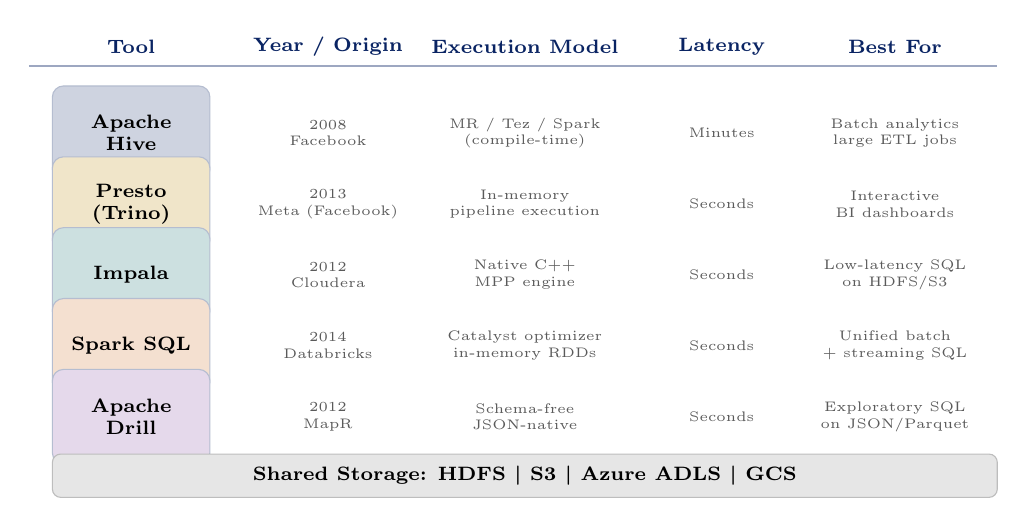
\begin{tikzpicture}[
      tool/.style={rectangle, rounded corners=4pt, minimum width=2.0cm,
                   minimum height=1.2cm, font=\scriptsize\bfseries, align=center,
                   draw=PUNavy!30},
      lbl/.style={font=\tiny, PUGray, align=center},
      hdr/.style={font=\scriptsize\bfseries, PUNavy}
    ]
    % Header row
    \node[hdr] at (-4.5, 3.3) {Tool};
    \node[hdr] at (-2.0, 3.3) {Year / Origin};
    \node[hdr] at (0.5,  3.3) {Execution Model};
    \node[hdr] at (3.0,  3.3) {Latency};
    \node[hdr] at (5.2,  3.3) {Best For};
    \draw[thick, PUNavy!40] (-5.8, 3.05) -- (6.5, 3.05);

    % Hive
    \node[tool, fill=PUNavy!20]   at (-4.5, 2.2) {Apache\\Hive};
    \node[lbl] at (-2.0, 2.2) {2008\\Facebook};
    \node[lbl] at (0.5,  2.2) {MR / Tez / Spark\\(compile-time)};
    \node[lbl] at (3.0,  2.2) {Minutes};
    \node[lbl] at (5.2,  2.2) {Batch analytics\\large ETL jobs};

    % Presto
    \node[tool, fill=PUGold!25]   at (-4.5, 1.3) {Presto\\(Trino)};
    \node[lbl] at (-2.0, 1.3) {2013\\Meta (Facebook)};
    \node[lbl] at (0.5,  1.3) {In-memory\\pipeline execution};
    \node[lbl] at (3.0,  1.3) {Seconds};
    \node[lbl] at (5.2,  1.3) {Interactive\\BI dashboards};

    % Impala
    \node[tool, fill=PUTeal!20]   at (-4.5, 0.4) {Impala};
    \node[lbl] at (-2.0, 0.4) {2012\\Cloudera};
    \node[lbl] at (0.5,  0.4) {Native C++\\MPP engine};
    \node[lbl] at (3.0,  0.4) {Seconds};
    \node[lbl] at (5.2,  0.4) {Low-latency SQL\\on HDFS/S3};

    % Spark SQL
    \node[tool, fill=PUOrange!20] at (-4.5, -0.5) {Spark SQL};
    \node[lbl] at (-2.0, -0.5) {2014\\Databricks};
    \node[lbl] at (0.5,  -0.5) {Catalyst optimizer\\in-memory RDDs};
    \node[lbl] at (3.0,  -0.5) {Seconds};
    \node[lbl] at (5.2,  -0.5) {Unified batch\\+ streaming SQL};

    % Drill
    \node[tool, fill=PUPurple!15] at (-4.5, -1.4) {Apache\\Drill};
    \node[lbl] at (-2.0, -1.4) {2012\\MapR};
    \node[lbl] at (0.5,  -1.4) {Schema-free\\JSON-native};
    \node[lbl] at (3.0,  -1.4) {Seconds};
    \node[lbl] at (5.2,  -1.4) {Exploratory SQL\\on JSON/Parquet};

    % Common storage substrate
    \node[rectangle, fill=PUGray!15, draw=PUGray!40, rounded corners=3pt,
          minimum width=12.0cm, minimum height=0.55cm,
          font=\scriptsize\bfseries, align=center]
          at (0.5, -2.15) {Shared Storage: HDFS \textbar\ S3 \textbar\ Azure ADLS \textbar\ GCS};
  \end{tikzpicture}
  \end{center}
\end{frame}

%================================================================
\section{Apache Hive Architecture}
%================================================================

\begin{frame}{Hive Architecture: From HiveQL to HDFS}
  \begin{columns}[T]
    \column{0.50\textwidth}
      \begin{block}{Component Roles}
        {\small
        \begin{itemize}
          \item \textbf{HiveServer2}: JDBC/ODBC server; authenticates users; accepts HiveQL queries from Beeline CLI, BI tools (Tableau, Power BI), and JDBC drivers
          \item \textbf{Driver}: core query processing pipeline — Parser $\to$ Semantic Analyser $\to$ Logical Planner $\to$ Query Optimizer $\to$ Physical Plan Generator
          \item \textbf{Metastore}: relational database (MySQL / PostgreSQL) storing all metadata: table schemas, column types, partition information, file locations on HDFS
          \item \textbf{Execution Engine}: pluggable — can be \textbf{MapReduce} (default legacy), \textbf{Tez} (DAG of tasks, faster), or \textbf{Spark} (\texttt{SET hive.execution.engine=spark})
          \item \textbf{HDFS}: actual data storage — Hive tables are directories; partitions are sub-directories
        \end{itemize}
        }
      \end{block}

    \column{0.47\textwidth}
      \begin{center}
      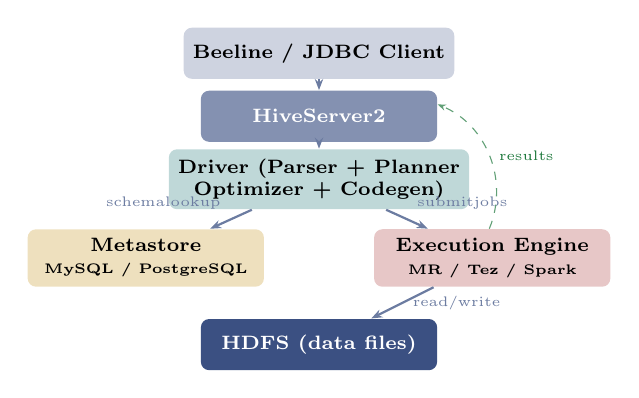
\begin{tikzpicture}[
          box/.style={rectangle, rounded corners=3pt, minimum width=3.0cm,
                      minimum height=0.65cm, font=\scriptsize\bfseries, align=center},
          arr/.style={-{Stealth[length=4pt]}, thick, PUNavy!60}
        ]
        \node[box, fill=PUNavy!20]        (cli)  at (0, 5.2) {Beeline / JDBC Client};
        \node[box, fill=PUNavy!50, text=white] (hs2) at (0, 4.4)
              {HiveServer2};
        \node[box, fill=PUTeal!25]        (drv)  at (0, 3.6)
              {Driver (Parser + Planner\\Optimizer + Codegen)};
        \node[box, fill=PUGold!30]        (meta) at (-2.2, 2.6)
              {Metastore\\{\tiny MySQL / PostgreSQL}};
        \node[box, fill=PURed!25]         (exec) at (2.2, 2.6)
              {Execution Engine\\{\tiny MR / Tez / Spark}};
        \node[box, fill=PUNavy!80, text=white] (hdfs) at (0, 1.5)
              {HDFS (data files)};

        \draw[arr] (cli)--(hs2);
        \draw[arr] (hs2)--(drv);
        \draw[arr] (drv) -- (meta)
              node[midway, above left, font=\tiny]{schema\\lookup};
        \draw[arr] (drv) -- (exec)
              node[midway, above right, font=\tiny]{submit\\jobs};
        \draw[arr] (exec)--(hdfs)
              node[midway, right, font=\tiny]{read/write};

        % Result path
        \draw[-{Stealth[length=3pt]}, PUGreen!70, dashed, bend right=45]
              (exec) to node[right, font=\tiny, PUGreen]{results} (hs2);
      \end{tikzpicture}
      \end{center}
  \end{columns}
\end{frame}

%----------------------------------------------------------------
\begin{frame}{The Hive Metastore: The Control Plane of Your Data Lake}
  \begin{columns}[T]
    \column{0.52\textwidth}
      \begin{block}{What the Metastore Stores}
        The Metastore is a \textbf{relational database} (typically MySQL or PostgreSQL) that acts as the \textbf{central catalogue} for all structured data on HDFS:
        \vspace{4pt}
        \begin{itemize}
          \item \textbf{Database \& Table definitions}: column names, data types, comment descriptions
          \item \textbf{Partition metadata}: which partition values exist (e.g., \texttt{year=2024, month=1}) and the HDFS path for each partition directory
          \item \textbf{SerDe (Serializer/Deserializer)}: how to parse the physical file format (ORC, Parquet, CSV, JSON) into column values
          \item \textbf{Table statistics}: row counts, column min/max, NULL counts (used by the query optimizer)
          \item \textbf{Privileges}: table-level and column-level access control
        \end{itemize}
      \end{block}

    \column{0.45\textwidth}
      \begin{alertblock}{Why the Metastore is Critical}
        \small Without the Metastore, Hive cannot answer a single query — it needs to know \textit{where} the data lives on HDFS and \textit{how} to parse it.  This is why the Metastore is often deployed as a \textbf{highly available service} (Metastore HA) in production clusters.
      \end{alertblock}
      \vspace{6pt}
      \begin{exampleblock}{Spotify Scale}
        \small Spotify's Hive Metastore catalogs over \textbf{1 million tables} across a cluster processing 600 billion events per day.  The Metastore itself runs on a replicated MySQL cluster with automatic failover.
        \vspace{4pt}
        \textbf{Lesson:} The Metastore is as important as HDFS itself.  Metastore corruption = inability to query any table even though data on HDFS is intact.
      \end{exampleblock}
  \end{columns}
\end{frame}

%================================================================
\section{Schema-on-Read vs.\ Schema-on-Write}
%================================================================

\begin{frame}{Schema-on-Read vs.\ Schema-on-Write}
  \begin{center}
  \renewcommand{\arraystretch}{1.5}
  \begin{tabular}{p{3.0cm}p{4.8cm}p{4.8cm}}
    \toprule
    \textbf{Property}     & \textbf{Schema-on-Write (RDBMS)} & \textbf{Schema-on-Read (Hive)} \\
    \midrule
    When schema enforced  & At INSERT / LOAD time             & At SELECT / query time \\
    Invalid data handling & \alert{Rejected immediately}       & Stored; NULL returned at query time \\
    Flexibility           & Rigid: must define schema upfront  & Flexible: schema applied to any file \\
    Write speed           & Slower (validation overhead)       & Fast: raw file copy to HDFS \\
    Query speed           & Faster (data pre-validated)        & Slower (parse \& validate per query) \\
    Multiple schemas      & One schema per table               & \textbf{Many schemas on same data} \\
    Storage format        & Proprietary (InnoDB pages)         & Open: ORC, Parquet, CSV, JSON, Avro \\
    Use case              & OLTP: e-commerce orders, banking   & OLAP: log analysis, batch reporting \\
    \midrule
    \textbf{Example}      & MySQL: \texttt{INSERT} fails if \texttt{amount} is text & Hive: stores ``abc'' in amount column; query returns \texttt{NULL} \\
    \bottomrule
  \end{tabular}
  \end{center}
  \vspace{4pt}
  \begin{columns}[T]
    \column{0.48\textwidth}
      \begin{block}{Schema-on-Read Advantage}
        \small Load raw web logs immediately to HDFS without knowing the final schema.  Define multiple different Hive tables over the same log files as requirements evolve.  No ETL transformation needed at ingest time.
      \end{block}
    \column{0.48\textwidth}
      \begin{alertblock}{Schema-on-Read Risk}
        \small Data quality issues are silent until query time.  A corrupted column returns NULL rather than an error.  Production data pipelines should combine schema-on-read Hive with downstream validation (Great Expectations, dbt tests) to catch bad data.
      \end{alertblock}
  \end{columns}
\end{frame}

%================================================================
\section{HiveQL: Syntax, Partitioning, and Bucketing}
%================================================================

\begin{frame}{HiveQL vs.\ SQL: Key Differences}
  \begin{center}
  \renewcommand{\arraystretch}{1.55}
  \begin{tabular}{p{3.0cm}p{4.2cm}p{4.2cm}}
    \toprule
    \textbf{Feature}    & \textbf{SQL (RDBMS)} & \textbf{HiveQL} \\
    \midrule
    Schema enforcement  & On write (strict)      & On read (flexible) \\
    ACID transactions   & Full: INSERT, UPDATE, DELETE, ROLLBACK & Limited: ORC tables with ACID mode only \\
    UPDATE / DELETE     & Any row, any time      & Only in ACID-enabled transactional tables \\
    Indexing            & B-tree, hash, bitmap   & Partitions + Buckets (no traditional indexes) \\
    Sub-queries         & Correlated sub-queries  & Non-correlated only (some limitations) \\
    Query latency       & Milliseconds           & Minutes (batch MapReduce) / Seconds (Tez/Spark) \\
    Execution model     & Single-node or MPP     & Distributed: MR / Tez / Spark DAG \\
    Data location       & Database storage engine & HDFS directories (user-managed) \\
    Scale               & Terabytes max          & Petabytes \\
    \midrule
    \textbf{Suitable workload} & OLTP (real-time reads/writes) & OLAP (batch analytics, reporting) \\
    \bottomrule
  \end{tabular}
  \end{center}
  \vspace{4pt}
  \begin{alertblock}{Exam Tip: The Most Common Misconception}
    \small Students often assume HiveQL = SQL and expect millisecond query response.  Hive is a \textbf{batch system}: a simple \texttt{SELECT COUNT(*)} on a 1 TB table may take 5--10 minutes on MapReduce.  Use Presto or Spark SQL for interactive latency.
  \end{alertblock}
\end{frame}

%----------------------------------------------------------------
\begin{frame}[fragile]{HiveQL: Table Creation and Basic Queries}
  \begin{columns}[T]
    \column{0.50\textwidth}
      \begin{exampleblock}{Creating and Loading a Table}
        \begin{lstlisting}
-- External table: data stays in HDFS
-- even if table is dropped
CREATE EXTERNAL TABLE transactions (
  txn_id   BIGINT,
  user_id  STRING,
  amount   DOUBLE,
  country  STRING,
  txn_date DATE
)
ROW FORMAT DELIMITED
  FIELDS TERMINATED BY ','
STORED AS ORC
LOCATION '/data/bkash/txns/';

-- Load data (moves file to table dir)
LOAD DATA INPATH
  '/staging/txns_2024.orc'
  INTO TABLE transactions;
        \end{lstlisting}
      \end{exampleblock}

    \column{0.47\textwidth}
      \begin{exampleblock}{HiveQL Aggregation Queries}
        \begin{lstlisting}
-- Top 5 countries by total amount
SELECT   country,
         SUM(amount) AS total_BDT
FROM     transactions
WHERE    YEAR(txn_date) = 2024
GROUP BY country
ORDER BY total_BDT DESC
LIMIT    5;

-- Monthly revenue trend
SELECT   MONTH(txn_date) AS mo,
         COUNT(*)        AS num_txns,
         AVG(amount)     AS avg_amount
FROM     transactions
WHERE    country = 'BD'
  AND    YEAR(txn_date) = 2024
GROUP BY MONTH(txn_date)
ORDER BY mo;
        \end{lstlisting}
      \end{exampleblock}
  \end{columns}
\end{frame}

%----------------------------------------------------------------
\begin{frame}{Partitioning: Directory-Level Data Pruning}
  \begin{columns}[T]
    \column{0.52\textwidth}
      \begin{block}{What Is Partitioning?}
        Partitioning physically organises table data into \textbf{separate HDFS sub-directories} based on the values of one or more columns.  When a query filters on the partition key, Hive reads \textbf{only the matching sub-directories} — skipping all others.
        \vspace{4pt}
        \begin{itemize}
          \item \textbf{Partition key}: typically a low-cardinality column used frequently in \texttt{WHERE} (date, country, region, status)
          \item \textbf{Benefit}: avoids full-table scan; reduces data read from HDFS; cuts job time proportionally
          \item \textbf{Example}: query on \texttt{year=2024, month=01} reads only 1 sub-directory, not 36 months of data
        \end{itemize}
      \end{block}
      \vspace{4pt}
      \begin{alertblock}{Partition Explosion Risk}
        \small Never partition on high-cardinality columns (e.g., \texttt{user\_id}, \texttt{txn\_id}).  A 100 M user table would create 100 M HDFS directories — crashing the NameNode with metadata overflow.
      \end{alertblock}

    \column{0.45\textwidth}
      \begin{center}
      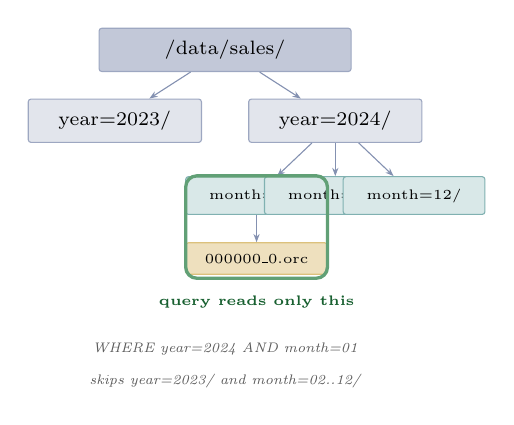
\begin{tikzpicture}[
          dir/.style={rectangle, draw=PUNavy!40, fill=PUNavy!12,
                      minimum width=2.2cm, minimum height=0.55cm,
                      font=\scriptsize, rounded corners=1pt},
          subd/.style={rectangle, draw=PUTeal!50, fill=PUTeal!15,
                       minimum width=1.8cm, minimum height=0.48cm,
                       font=\tiny, rounded corners=1pt},
          arr/.style={-{Stealth[length=3pt]}, PUNavy!50}
        ]
        % Root table dir
        \node[dir, minimum width=3.2cm, fill=PUNavy!25]
              (root) at (0, 4.5) {/data/sales/};
        % Year partitions
        \node[dir] (y23) at (-1.4, 3.6) {year=2023/};
        \node[dir] (y24) at ( 1.4, 3.6) {year=2024/};
        \draw[arr] (root)--(y23);
        \draw[arr] (root)--(y24);
        % Month partitions under year=2024
        \node[subd] (m01) at (0.4, 2.65)  {month=01/};
        \node[subd] (m02) at (1.4, 2.65)  {month=02/};
        \node[subd] (m12) at (2.4, 2.65)  {month=12/};
        \draw[arr] (y24)--(m01);
        \draw[arr] (y24)--(m02);
        \draw[arr] (y24)--(m12);
        % ORC files inside month=01
        \node[rectangle, fill=PUGold!30, draw=PUGold!60,
              font=\tiny, rounded corners=1pt,
              minimum width=1.8cm, minimum height=0.4cm]
              (orc) at (0.4, 1.85) {000000\_0.orc};
        \draw[arr] (m01)--(orc);
        % Highlight / query
        \draw[very thick, PUGreen!70, rounded corners=4pt]
              (-0.5, 1.6) rectangle (1.3, 2.9);
        \node[font=\tiny\bfseries, PUGreen!80!black] at (0.4, 1.3)
              {query reads only this};

        % Legend
        \node[font=\tiny\itshape, PUGray] at (0, 0.7)
              {WHERE year=2024 AND month=01};
        \node[font=\tiny\itshape, PUGray] at (0, 0.3)
              {skips year=2023/ and month=02..12/};
      \end{tikzpicture}
      \end{center}
  \end{columns}
\end{frame}

%----------------------------------------------------------------
\begin{frame}[fragile]{Partitioning: DDL and Dynamic Partition Insert}
  \begin{columns}[T]
    \column{0.50\textwidth}
      \begin{exampleblock}{Creating a Partitioned Table}
        \begin{lstlisting}
CREATE TABLE sales (
  txn_id  BIGINT,
  amount  DOUBLE,
  country STRING
)
PARTITIONED BY (year INT, month INT)
STORED AS ORC;

-- Static partition load
INSERT INTO sales
  PARTITION (year=2024, month=1)
SELECT txn_id, amount, country
FROM   raw_sales
WHERE  sale_year = 2024
  AND  sale_month = 1;
        \end{lstlisting}
      \end{exampleblock}
      \vspace{4pt}
      \begin{block}{Query Pruning in Action}
        \begin{lstlisting}
-- Hive reads ONLY year=2024/month=1/
-- Skips all other partitions
SELECT SUM(amount)
FROM   sales
WHERE  year=2024 AND month=1;
        \end{lstlisting}
      \end{block}

    \column{0.47\textwidth}
      \begin{exampleblock}{Dynamic Partition Insert (all months at once)}
        \begin{lstlisting}
-- Enable dynamic partitioning
SET hive.exec.dynamic.partition=true;
SET hive.exec.dynamic.partition.mode
    =nonstrict;

-- Hive infers partition values
-- from the last SELECT columns
INSERT INTO sales
  PARTITION (year, month)
SELECT txn_id,
       amount,
       country,
       YEAR(sale_date)  AS year,
       MONTH(sale_date) AS month
FROM   raw_sales;
        \end{lstlisting}
      \end{exampleblock}
      \vspace{4pt}
      \begin{alertblock}{Rule}
        \small Partition columns must appear \textbf{last} in the SELECT list when using dynamic partition INSERT.  If you specify \texttt{PARTITION (year, month)} but select \texttt{month} before \texttt{year}, Hive silently assigns values incorrectly.
      \end{alertblock}
  \end{columns}
\end{frame}

%----------------------------------------------------------------
\begin{frame}{Bucketing: Hash-Based Clustering for Efficient JOINs}
  \begin{columns}[T]
    \column{0.52\textwidth}
      \begin{block}{What Is Bucketing?}
        Bucketing further divides each partition into a \textbf{fixed number of files} (buckets) using a \textbf{hash function} on a chosen column.  Rows with the same hash(column) land in the same bucket file.
        \vspace{4pt}
        \begin{enumerate}
          \item Define \texttt{CLUSTERED BY (column) INTO N BUCKETS}
          \item All rows where \texttt{hash(column) \% N = k} are written to bucket file \texttt{k}
          \item Result: same bucket file across two tables contains rows that \textbf{will join together}
        \end{enumerate}
        \vspace{4pt}
        \textbf{Bucket Map Join} (the main benefit):
        \begin{itemize}
          \item Both tables bucketed on join key with the \textbf{same number of buckets}
          \item Hive can JOIN bucket 0 of table A with bucket 0 of table B, bucket 1 with bucket 1, etc.
          \item \textbf{No full sort-merge shuffle} needed — massive speedup vs.\ un-bucketed JOIN
        \end{itemize}
      \end{block}

    \column{0.45\textwidth}
      \begin{center}
      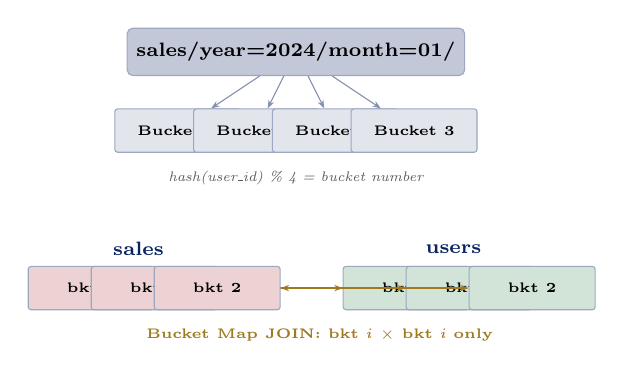
\begin{tikzpicture}[
          bkt/.style={rectangle, draw=PUNavy!40, fill=PUNavy!12,
                      minimum width=1.6cm, minimum height=0.55cm,
                      font=\tiny\bfseries, rounded corners=1pt},
          arr/.style={-{Stealth[length=3pt]}, PUNavy!50}
        ]
        % Partition dir
        \node[rectangle, fill=PUNavy!25, draw=PUNavy!40,
              font=\scriptsize\bfseries, rounded corners=2pt,
              minimum width=4.2cm, minimum height=0.6cm]
              (part) at (0, 4.0) {sales/year=2024/month=01/};
        % Buckets
        \foreach \i/\x in {0/-1.5, 1/-0.5, 2/0.5, 3/1.5} {
          \node[bkt] (b\i) at (\x, 3.0) {Bucket \i};
          \draw[arr] (part)--(b\i);
        }
        % Hash explanation
        \node[font=\tiny\itshape, PUGray] at (0, 2.4)
              {hash(user\_id) \% 4 = bucket number};

        % Two tables joining
        \node[font=\scriptsize\bfseries, PUNavy] at (-2.0, 1.5)
              {sales};
        \node[font=\scriptsize\bfseries, PUNavy] at (2.0, 1.5)
              {users};
        \foreach \i/\xa/\xb in {0/-2.6/1.4, 1/-1.8/2.2, 2/-1.0/3.0} {
          \node[bkt, fill=PURed!20]  (sa\i) at (\xa, 1.0) {bkt \i};
          \node[bkt, fill=PUGreen!20] (ub\i) at (\xb, 1.0) {bkt \i};
          \draw[{Stealth[length=3pt]}-{Stealth[length=3pt]},
                PUGold!80!black, thick] (sa\i)--(ub\i);
        }
        \node[font=\tiny\bfseries, PUGold!80!black] at (0.3, 0.4)
              {Bucket Map JOIN: bkt \textit{i} $\times$ bkt \textit{i} only};
      \end{tikzpicture}
      \end{center}
      \vspace{4pt}
      \begin{exampleblock}{Bucketing DDL}
        {\scriptsize\texttt{CLUSTERED BY (user\_id) INTO 32 BUCKETS STORED AS ORC;}}
      \end{exampleblock}
  \end{columns}
\end{frame}

%================================================================
\section{Presto: Interactive SQL on Hadoop}
%================================================================

\begin{frame}{Presto: In-Memory SQL, 10$\times$ Faster than Hive+MapReduce}
  \begin{columns}[T]
    \column{0.52\textwidth}
      \begin{block}{Why Presto Was Built (Meta, 2013)}
        Facebook analysts needed \textbf{interactive} (sub-second to second) SQL queries over petabytes of data on HDFS.  Hive+MapReduce could not deliver this — even a simple filtered \texttt{COUNT} took minutes.
        \vspace{4pt}
        \textbf{Presto key design decisions:}
        \begin{enumerate}
          \item \textbf{No intermediate disk writes}: data flows as a pipeline through the cluster entirely in memory
          \item \textbf{Vectorized execution}: processes column chunks (batches of 1{,}024 rows) rather than row by row
          \item \textbf{Cost-based optimizer}: uses table statistics to choose optimal join order and join strategy
          \item \textbf{Connector architecture}: same SQL engine for HDFS, Hive, Cassandra, MySQL, Kafka, and S3 simultaneously in one query
        \end{enumerate}
      \end{block}

    \column{0.45\textwidth}
      \begin{center}
      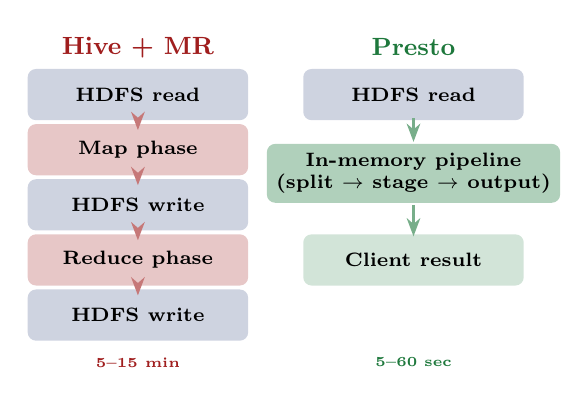
\begin{tikzpicture}[
          box/.style={rectangle, rounded corners=3pt, minimum width=2.8cm,
                      minimum height=0.65cm, font=\scriptsize\bfseries, align=center},
          arr/.style={-{Stealth[length=4pt]}, thick}
        ]
        % Hive path
        \node[font=\small\bfseries, PURed] at (-1.5, 4.2) {Hive + MR};
        \node[box, fill=PUNavy!20]  at (-1.5, 3.6) {HDFS read};
        \node[box, fill=PURed!25]   at (-1.5, 2.9) {Map phase};
        \node[box, fill=PUNavy!20]  at (-1.5, 2.2) {HDFS write};
        \node[box, fill=PURed!25]   at (-1.5, 1.5) {Reduce phase};
        \node[box, fill=PUNavy!20]  at (-1.5, 0.8) {HDFS write};
        \node[font=\tiny\bfseries, PURed] at (-1.5, 0.2) {5--15 min};

        \draw[-{Stealth}, PURed!60, thick] (-1.5,3.3)--(-1.5,3.15);
        \draw[-{Stealth}, PURed!60, thick] (-1.5,2.6)--(-1.5,2.45);
        \draw[-{Stealth}, PURed!60, thick] (-1.5,1.9)--(-1.5,1.75);
        \draw[-{Stealth}, PURed!60, thick] (-1.5,1.2)--(-1.5,1.05);

        % Presto path
        \node[font=\small\bfseries, PUGreen] at (2.0, 4.2) {Presto};
        \node[box, fill=PUNavy!20]  at (2.0, 3.6) {HDFS read};
        \node[box, fill=PUGreen!35] at (2.0, 2.6)
              {In-memory pipeline\\(split $\to$ stage $\to$ output)};
        \node[box, fill=PUGreen!20] at (2.0, 1.5) {Client result};
        \node[font=\tiny\bfseries, PUGreen] at (2.0, 0.2) {5--60 sec};

        \draw[-{Stealth}, PUGreen!60, thick] (2.0,3.3)--(2.0,3.0);
        \draw[-{Stealth}, PUGreen!60, thick] (2.0,2.2)--(2.0,1.8);
      \end{tikzpicture}
      \end{center}
  \end{columns}
  \vspace{4pt}
  \begin{exampleblock}{When to Use Which}
    \small \textbf{Use Hive} for large ETL jobs ($>$1 TB transformations), nightly batch pipelines, and jobs that span hours.  \textbf{Use Presto/Trino} for interactive analyst queries, BI dashboards, and ad-hoc exploration where waiting minutes is unacceptable.
  \end{exampleblock}
\end{frame}

%================================================================
\section{Ivy League Alignment}
%================================================================

\begin{frame}{Hive \& SQL-on-Hadoop in Top University Curricula}
  \begin{columns}[T]
    \column{0.55\textwidth}
      \begin{block}{Stanford CS246 — Mining of Massive Datasets}
        \small Stanford frames Hive as the canonical example of \textbf{declarative MapReduce} — the same principle as relational algebra on distributed data:
        \begin{itemize}
          \item HiveQL's \texttt{GROUP BY} + aggregation compiles to a MapReduce job where Map emits (key, value) pairs and Reduce applies the aggregate function — \textit{this is the Relational Algebra $\gamma$ operator distributed}
          \item CS246 assignment: \textbf{write a matrix multiply in HiveQL} and compare to raw MapReduce implementation — motivating why SQL abstractions matter even for non-relational computations
          \item \textbf{Exam question type}: \textit{``Given a HiveQL query with two JOINs and a GROUP BY, draw the MapReduce DAG that Hive would generate, identifying the shuffle key at each stage.''}
        \end{itemize}
      \end{block}

    \column{0.42\textwidth}
      \begin{exampleblock}{MIT 6.830 — Database Systems}
        \small MIT covers Hive as a \textbf{bridge between traditional RDBMS and distributed systems}:
        \begin{itemize}
          \item Schema-on-read vs.\ schema-on-write is a core concept in MIT's coverage of data lakes
          \item The Hive Metastore is compared to PostgreSQL's \texttt{pg\_catalog} — both are the system catalogue, but Hive's operates over HDFS
          \item MIT students implement a simplified Hive planner that converts SQL parse trees into MapReduce job chains
        \end{itemize}
      \end{exampleblock}
      \vspace{4pt}
      \begin{alertblock}{CMU 15-721 — Advanced DB Systems}
        \small CMU benchmarks Hive, Presto, Impala, and Spark SQL on the TPC-DS benchmark (99 complex SQL queries over 3 TB).  Presto wins on latency; Hive wins on throughput for batch ETL.  CMU uses this to teach \textbf{the query optimizer as the differentiating layer}.
      \end{alertblock}
  \end{columns}
\end{frame}

%================================================================
\section{Student Assessment Pool}
%================================================================

\begin{frame}{Assessment\textemdash MCQ Set A \hfill\small\textit{CLO3, CLO4}}
  \begin{exampleblock}{Instructions}
    Select the single best answer.  Correct answers \textbf{bolded} for instructor reference.
  \end{exampleblock}
  \vspace{8pt}
  \begin{itemize}
    \item[\textbf{Q1.}] In Hive, where is table schema metadata (column names, types, partition info) stored?
    \begin{enumerate}[(a)]
      \item HDFS NameNode
      \item \textbf{Hive Metastore (relational DB such as MySQL)}
      \item HBase
      \item ZooKeeper
    \end{enumerate}
  \end{itemize}
  \vspace{8pt}
  \begin{itemize}
    \item[\textbf{Q2.}] What does ``schema-on-read'' mean in the context of Hive?
    \begin{enumerate}[(a)]
      \item Schema is validated when data is inserted into the table
      \item \textbf{Schema is applied when data is queried, not when it is stored on HDFS}
      \item Schema is stored separately from data in HDFS metadata
      \item Schema is inferred automatically from column names in the file header
    \end{enumerate}
  \end{itemize}
  \vspace{8pt}
  \begin{alertblock}{Instructor Notes}
    \textbf{Q1:} A common distractor is the NameNode --- it stores HDFS block metadata, not table schemas.  \textbf{Q2:} Option (d) describes schema inference (like CSV auto-detect in Spark), which is different from schema-on-read: in schema-on-read the user explicitly defines the schema at query time (via \texttt{CREATE TABLE}).
  \end{alertblock}
\end{frame}

%----------------------------------------------------------------
\begin{frame}{Assessment\textemdash MCQ Set B \hfill\small\textit{CLO3, CLO4}}
  \vspace{6pt}
  \begin{itemize}
    \item[\textbf{Q3.}] Which Hive optimization technique physically organises data into separate HDFS sub-directories by a column's value to avoid full table scans?
    \begin{enumerate}[(a)]
      \item Bucketing \quad (b) Indexing \quad (c) \textbf{Partitioning} \quad (d) Compression
    \end{enumerate}
  \end{itemize}
  \vspace{8pt}
  \begin{itemize}
    \item[\textbf{Q4.}] Presto's primary performance advantage over Hive+MapReduce for interactive queries is:
    \begin{enumerate}[(a)]
      \item Presto supports more SQL functions than HiveQL
      \item Presto has better native integration with HBase and Cassandra
      \item \textbf{Presto executes queries entirely in memory without writing intermediate results to disk}
      \item Presto has native Python UDF support
    \end{enumerate}
  \end{itemize}
  \vspace{8pt}
  \begin{alertblock}{Instructor Notes}
    \textbf{Q3:} Bucketing (a) divides \textit{within} a partition by hash --- it reduces join cost but does not skip data at the directory level.  \textbf{Q4:} The key word is ``intermediate results to disk.''  Hive+MapReduce materialises intermediate data to HDFS between every MapReduce stage.  Presto pipelines everything in memory, eliminating this I/O completely for most queries.
  \end{alertblock}
\end{frame}

%----------------------------------------------------------------
\begin{frame}{Assessment\textemdash True / False \hfill\small\textit{CLO3, CLO4}}
  \begin{block}{Instructions}
    State True or False and provide a \textbf{one-sentence justification} for full marks.
  \end{block}
  \vspace{6pt}
  \centering
  \renewcommand{\arraystretch}{1.6}
  \begin{tabular}{p{9.0cm}c}
    \toprule
    \textbf{Statement} & \textbf{Answer} \\
    \midrule
    1.\ HiveQL supports full ACID transactions on all table types, just like MySQL. &
    \alert{\textbf{False}} \\
    2.\ Partitioning in Hive reduces query time by eliminating irrelevant data partitions from the HDFS scan. &
    \textbf{True} \\
    3.\ Hive directly executes a HiveQL query on HDFS without any intermediate translation step. &
    \alert{\textbf{False}} \\
    4.\ Bucketing in Hive is particularly useful for optimising JOIN operations between two large tables. &
    \textbf{True} \\
    \bottomrule
  \end{tabular}
  \vspace{6pt}
  \begin{exampleblock}{Model Justifications}
    \small \textbf{1:} ACID is only available on ORC-backed transactional tables with explicit \texttt{TBLPROPERTIES (``transactional''=``true'')}.  \textbf{3:} Hive's Driver parses HiveQL, creates a logical plan, optimises it, and compiles it into a \textbf{DAG of MapReduce, Tez, or Spark jobs} before any data is touched.  \textbf{4:} Bucket map joins match corresponding bucket numbers (same hash), avoiding a full shuffle-sort phase.
  \end{exampleblock}
\end{frame}

%----------------------------------------------------------------
\begin{frame}{Assessment\textemdash Descriptive Questions \hfill\small\textit{CLO3}}
  \begin{block}{Instructions}
    Answer each question in \textbf{100--150 words}.  Include a diagram where indicated.
  \end{block}
  \vspace{8pt}
  \begin{itemize}
    \item[\textbf{D1.}] Explain the \textbf{Hive architecture}: what is the role of HiveServer2, the Driver, and the Metastore?  How is a HiveQL query compiled into executable jobs?  Draw the component diagram.
  \end{itemize}
  \vspace{8pt}
  \begin{itemize}
    \item[\textbf{D2.}] Differentiate between \textbf{partitioning} and \textbf{bucketing} in Hive.  When would you choose each?  Describe a scenario in Bangladesh e-commerce data where both are used together.
  \end{itemize}
  \vspace{8pt}
  \begin{itemize}
    \item[\textbf{D3.}] What is ``\textbf{schema-on-read}''?  What are its advantages and disadvantages compared to ``schema-on-write'' in a traditional RDBMS such as MySQL?  Give one example where schema-on-read causes a data quality problem.
  \end{itemize}
\end{frame}

%----------------------------------------------------------------
\begin{frame}[fragile]{Assessment\textemdash Analytical Questions \hfill\small\textit{CLO4}}
  \begin{block}{Instructions}
    Answer in \textbf{200--300 words} with step-by-step reasoning and HiveQL code where applicable.
  \end{block}
  \vspace{6pt}
  \begin{itemize}
    \item[\textbf{A1.}] \textbf{Partitioning \& Bucketing Design:}\\
    You have a 5 TB e-commerce transaction table with columns: \texttt{(txn\_id, user\_id, product\_id, amount, country, txn\_date)}.  Design a complete partitioning and bucketing strategy to optimise:
    \begin{itemize}
      \item Daily revenue reports filtered by \texttt{country} and \texttt{txn\_date}
      \item JOINs between this table and a 10 M-row user profile table (keyed on \texttt{user\_id})
    \end{itemize}
    Write the complete \texttt{CREATE TABLE} DDL.  Justify why you chose a specific number of buckets and which column(s) you partitioned on.
  \end{itemize}
  \vspace{6pt}
  \begin{itemize}
    \item[\textbf{A2.}] \textbf{Query Compilation to MapReduce:}\\
    Write HiveQL to find the \textbf{top 5 products by total revenue in 2023}.  Then trace how Hive compiles this query into MapReduce stages: what is emitted by the Map phase, what is the shuffle key, and what does the Reduce phase compute?  How would switching the execution engine from MapReduce to Tez change the execution plan?
  \end{itemize}
\end{frame}

%================================================================
\section*{Textbook References}
%================================================================

\begin{frame}{Textbook \& Reading References}
  \begin{block}{Primary Textbooks for Week 7}
    \begin{itemize}
      \item \textbf{[TW]}\ Tom White. \textit{Hadoop: The Definitive Guide}, O'Reilly, 4th ed., 2015.
            \hfill \textbf{Ch.\ 12}
            \begin{itemize}
              \small\item Ch.\,12: Hive — comprehensive coverage of architecture, HiveQL, partitioning, bucketing, and UDFs
            \end{itemize}
      \item \textbf{[SA]}\ Acharya \& Chellappan. \textit{Big Data and Analytics}, Wiley, 2015.
            \hfill \textbf{Ch.\ 5}
            \begin{itemize}
              \small\item Ch.\,5: Apache Hive; data warehousing on Hadoop
            \end{itemize}
      \item \textbf{[LRU]}\ Leskovec, Rajaraman \& Ullman. \textit{Mining of Massive Datasets}, 3rd ed.
            \hfill \textbf{Ch.\ 2}
            \begin{itemize}
              \small\item Ch.\,2: SQL analogies in MapReduce; relational algebra in distributed systems
            \end{itemize}
    \end{itemize}
  \end{block}
  \vspace{6pt}
  \begin{exampleblock}{Seminal Papers (covered in Week 7, Part 2)}
    \begin{itemize}
      \small
      \item Thusoo, A.\ et al.\ (2009). \textbf{Hive -- A Warehousing Solution Over a Map-Reduce Framework.}
            \textit{PVLDB 2009.}
      \item Thusoo, A.\ et al.\ (2010). \textbf{Hive -- A Petabyte Scale Data Warehouse Using Hadoop.}
            \textit{IEEE ICDE 2010.}
      \item Venkataraman, S.\ et al.\ (2019). \textbf{Presto: SQL on Everything.}
            \textit{IEEE ICDE 2019.}
    \end{itemize}
  \end{exampleblock}
\end{frame}

%----------------------------------------------------------------
\begin{frame}[c]
  \begin{center}
    {\Large\bfseries Questions \& Discussion}\\[10pt]
    {\large Week 7, Part 1 $\;\mid\;$ CSE 4345 Big Data Analytics}\\[8pt]
    \textcolor{PUGray}{\rule{7cm}{0.5pt}}\\[10pt]
    \begin{quote}
      \itshape ``The key insight behind Hive is not the SQL syntax --- it is the Metastore: a shared, persistent catalogue that decouples the \textit{schema} of your data from the \textit{files} that hold it.''
    \end{quote}
    \hfill\textemdash\ Adapted from Thusoo et al., ICDE 2010
    \vspace{12pt}
    \begin{block}{\centering Next Lecture: Week 7, Part 2}
      \centering
      Seminal Papers: Thusoo et al.\ (2009, 2010) on Hive architecture and petabyte-scale warehousing\\[4pt]
      Case Study: \textbf{Spotify's Hive-Based Analytics Platform} ---
      1 million tables, 600 billion events/day, artist royalty reporting at scale
    \end{block}
    \vspace{6pt}
    \textbf{Reading before Part 2:}\ \textbf{[TW]} Ch.\,12 $\cdot$ Thusoo et al.\ (2009) PVLDB paper (see references)
  \end{center}
\end{frame}

%=================================================================
\end{document}
%=================================================================
